\title{Internet of Things}
\subtitle{Grundlagen des Internet of Things}
\institute{DHBW Karlsruhe, Mechatronik}
\author{Dennis Schulmeister-Zimolong}

\renewcommand{\ubInstitute}{Studiengang Mechatronik}
\renewcommand{\ubModule}{Internet of Things}
\renewcommand{\ubType}{Aufgaben}

%%% Folie: Vorstellung des Dozenten noch vor dem Inhaltsverzeichnis
\renewcommand{\IntroFrames} {
    \footnotesize

    \begin{frame}{Dennis Schulmeister-Zimolong}
        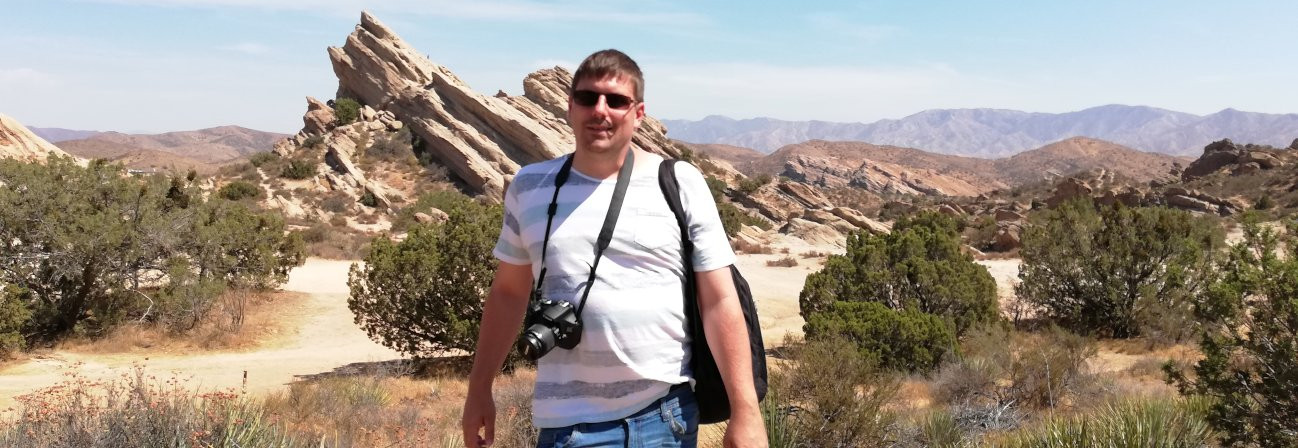
\includegraphics[width=\textwidth]{img/dozent_schulmeister}
        \vskip .5em

        \LinkButton{https://www.wpvs.de}{wpvs.de}
        \LinkButton{https://www.iot-embedded.de}{iot-embedded.de}
        \LinkButton{mailto:"Dennis Schulmeister-Zimolong" <dhbw@windows3.de>}{E-Mail}
        \vskip .8em

        \begin{itemize}
            \item Dipl.-Wirtschaftsinformatiker (DH), DHBW Karlsruhe, 2005 – 2008
            \item Produktmanager / Senior Entwickler für SAP Add-Ons, SOA People AG
            \item Seit 1992 begeistert von Computern und deren Programmierung
            \item Seit 2009 nebenberuflicher Dozent an der DHBW Karlsruhe
            \item Vorlesungen: Webprogrammierung, Verteilte Systeme, Internet of Things
            \item Keyboarder, Bassist, Sänger und Songwriter in der Freizeit
            \item Papa einer süßen kleinen Tochter \smiley{}
        \end{itemize}
    \end{frame}
}
